\section{Opis problemu}
\label{sec:problem}

Przedmiotem projektu jest znalezienie optymalnych parametrów maszyny wektorów nośnych (SVM-- \textit{Support Vector Machine}) w zagadnieniu aproksymacji. Aproksymowaną funkcją miała być dowolna ciągła funkcja dwuwymiarowa. W tym przypadku przyjęto funkcję określoną wzorem:

\begin{equation}
    \label{eqn:fun}
    f(x,y) = \log_{10}{|x|} \cos{y} + 0,55(x+y)
\end{equation}
\smallskip

\begin{figure}[h]
    \centering
    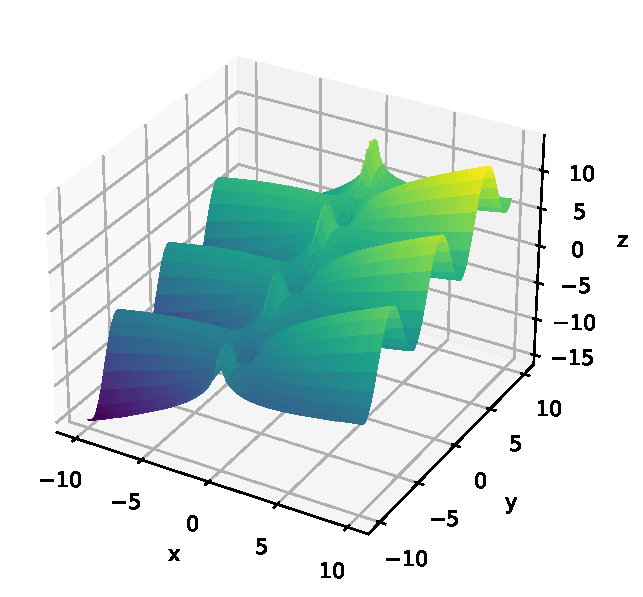
\includegraphics[width=0.5\textwidth]{assets/fun.pdf}
    \caption{Wykres aproksymowanej funkcji dwuwymiarowej}
    \label{fig:fun}
\end{figure}

W celu znalezienia optymalnych dla problemu parametrów zbadany zostanie wpływ poszczególnych parametrów algorytmu (funkcje jądrowe i ich atrybuty) na jakość regresji. Co więcej, aby sprawdzić, jak SVR (\textit{Support Vector Machine -- Regression}) poradziłby sobie dla rzeczywistych danych pomiarowych: zasymulowane zostaną one poprzez dodanie do aproksymowanej funkcji szumu. Zbadana zostanie jakość przybliżenia funkcji dla różnych poziomów szumu. Odporność przygotowanych modeli zostanie porównana z~innymi modelami regresji.

Jako miary oceny działania algorytmu wybrano:
\begin{itemize}
    \item błąd średniokwadratowy ($MSE$)
    \item średni błąd względny ($MAE$),
    \item współczynnik determinacji ($R^2$).
\end{itemize}

\begin{equation}
    \label{eqn:mse}
    MSE =\frac{1}{n} \sum_{i=1}^n (x_{i}-\hat{x}_{i})^2 \\[2ex]
\end{equation}
        
\begin{equation}
    \label{eqn:mae}
    MAE =\frac{1}{n} \sum_{i=1}^n \lvert x_{i}-\hat{x}_{i} \rvert \\[2ex]
\end{equation}
        
\begin{equation}
    \label{eqn:r2}
    R^{2} =1 - \frac{\sum_{i=1}^n (x_{i}-\hat{x}_{i})^2}{\sum_{i=1}^n (x_{i}-\bar{x}_{i})^2}   \\[2ex]
\end{equation}
        
\noindent
$\displaystyle
\begin{array}{ll}
              n      & \text{liczba pomiarów}\\
            x_{i} & \text{wartość rzeczywista}\\
            \hat{x}_{i} & \text{wartość przewidziana} \\
            \bar{x}_{i} & \text{wartość średnia} x
\end{array}
$